\section{Results}
\label{sec:result}

All simulations were performed with using Matlab and were run on a standard personal computer (Intel core i7, 16Go RAM). Reports of the execution times are omitted throughout, since the times are very short, due to the fact that the proposed models are ``na\"ive," \textit{i.e.}, there is no learning phase. 

\subsection{Specific Location}
\label{sec:ajaccio}
In this part, only the results obtained in France at the Ajaccio site (west coast of Corsica 41°55'36"N, 8°44'13"E, alt 30 m) for different forecast horizons are shown. The climate is Mediterranean, with mild, relatively rainy winters and hot, sunny summers, sometimes sultry, but tempered by the breeze ($KG=$ Csa). The site is in an area exposed to the Mistral wind, which blows from the Gulf of Lion. The average temperature of the coldest months (January, February) is 9 °C, that of the warmest months (July, August) 22.5 °C. The forecastability $F$ is estimated close to $68\%$ \citep{doi:10.1063/5.0042710}, which gives it climatic characteristics relative to cloudy occurrences (and thus to solar radiation) relatively straightforward to predict. 

It is important to verify the impact of the ratio to seasonal trend. According to Eq.(\ref{eq:24}) and considering a $90\%$ confidence level ($\alpha=0.1$), the quantile $q_{0.95}=1.645$. Computing $\rho$ with 100 data points ($n=100$) we obtain for global solar irradiation ($I_m$) $t(m)=0.4032$ and $\rho(m)=0.62$ while in the clear sky index case ($\kappa_m$), $t(m)=0.2918$  and $\rho(m)=0.1842$. The use of clear-sky series has a significant impact on seasonality, and we therefore consider that the predictive methodology described above can be applied, as soon as the ratio to trend ($I_{CS}$) is carried out.

Tables \ref{tab:1a} and \ref{tab:1b} show the error metrics related to prediction concerning horizon between 1 and 10 h. The presented models are persistence (PER in Section~\ref{sec:subsec1}), climatology (CLIM in Section~\ref{sec:subsec2}), climatology persistence (CLIPER or AR(1) in Section~\ref{sec:AR}), exponential smoothing (ES in Section~\ref{sec:ETS}), our proposed modified ARTU (or AR(2) in Section~\ref{sec:method}) and a combination of  CLIPER, ARTU (for $R=0.05$) PER and ES (COMB in Section~\ref{sec:comb}). The MASE is computed with $m=13$ and not 24 because the filtration of night hours reduces the number of data per day, depending on the day considered (time of year); the periodicity varies between 9 and 15 h on this site. 


\begin{table}[tb]
\begin{tabular}{@{}llcccccccccc@{}}\toprule
         &           & \multicolumn{10}{c}{Horizons (h)}                                                                                                                    \\  
         &           & 1             & 2             & 3             & 4             & 5             & 6             & 7             & 8             & 9             & 10            \\ \midrule
PER     & nRMSE     & 22.1          & 31.8          & 40.2          & 47.6          & 52.7          & 55.0          & 55.2          & 53.6          & 51.7          & 49.3          \\  
         & nMAE      & \textbf{11.9} & 17.6          & 21.7          & 25.1          & 27.6          & 29.3          & 30.1          & 30.3          & 29.9          & 29.2          \\ \addlinespace 
CLIM     & nRMSE     & 70.6          & 70.6          & 70.7          & 70.7          & 70.7          & 70.8          & 70.8          & 70.8          & 70.8          & 70.8          \\  
         & nMAE      & 60.7          & 60.8          & 60.8          & 60.8          & 60.9          & 60.9          & 60.9          & 61.0          & 61.0          & 61.0          \\ \addlinespace
CLIPER & nRMSE     & 21.3          & 27.7          & 30.5          & 32.5          & 33.6          & 34.0          & 34.3          & 34.5          & 34.7          & 34.8          \\  
         & nMAE      & 13.9          & 18.8          & 20.7          & 21.9          & 22.6          & 23.1          & 23.4          & 23.7          & 23.8          & 23.9          \\ \addlinespace 
ES       & nRMSE     & 22.4          & 30.3          & 33.5          & 35.5          & 36.9          & 37.0          & 36.6          & \textbf{34.4} & 36.6          & 36.9          \\  
         & nMAE      & 13.3          & 19.3          & 21.5          & 23.3          & 24.1          & 24.4          & 24.5          & 24.6          & 25.0          & 25.0          \\ \addlinespace 
ARTU     & nRMSE     & 22.2          & 30.8          & 30.7          & 32.4          & 33.5          & 34.0          & 34.3          & 34.4          & 34.7          & 34.8          \\  
R=0     & nMAE      & 14.8          & 21.3          & 20.9          & 27.8          & 22.7          & 23.2          & 23.5          & 23.6          & 23.8          & 23.9          \\ \addlinespace 
ARTU     & nRMSE     & 21.3          & 27.6          & 30.3          & \textbf{32.3} & \textbf{33.4} & \textbf{33.9} & 34.2          & 34.4          & \textbf{34.7} & 34.8          \\  
R=0.01  & nMAE      & 13.9          & 18.7          & 20.4          & 21.7          & 22.5          & 23.0          & \textbf{23.3} & \textbf{23.6} & \textbf{23.8} & \textbf{23.8} \\ \addlinespace 
ARTU     & nRMSE     & 21.3          & 27.5          & \textbf{30.3} & 32.3          & 33.4          & 33.9          & \textbf{34.2} & 34.5          & 34.7          & \textbf{34.8} \\  
R=0.05  & nMAE      & 13.9          & 18.6          & 20.4          & 21.7          & 22.5          & 23.0          & 23.3          & 23.6          & 23.8          & 23.8          \\ \addlinespace 
ARTU     & nRMSE     & 21.3          & 27.5          & 30.3          & 32.3          & 33.4          & 33.9          & 34.2          & 34.5          & 34.7          & 34.8          \\  
R=0.1   & nMAE      & 13.9          & 18.6          & 20.4          & 21.7          & \textbf{22.5} & \textbf{23.0} & 23.3          & 23.7          & 23.8          & 23.8          \\ \addlinespace 
COMB     & nRMSE     & \textbf{20.5} & \textbf{26.9} & 30.8          & 33.9          & 35.9          & 36.5          & 36.5          & 36.2          & 36.3          & 36.3          \\  
         & nMAE      & 12.4          & \textbf{17.2} & \textbf{19.5} & \textbf{21.3} & 22.6          & 23.2          & 23.6          & 23.8          & 24.0          & 24.0          \\ \bottomrule
\end{tabular}
\caption{nRMSE and nMAE for the six different benchmark methods at Ajaccio, France. The lowest error metrics values for each horizon are highlighted in bold.}\label{tab:1a}




\end{table}

% Please add the following required packages to your document preamble:
% \usepackage{booktabs}
% Please add the following required packages to your document preamble:
% \usepackage{booktabs}
\begin{table}[tb]
\centering

\begin{tabular}{@{}llccccccccc@{}}
\toprule
& PER  & CLIM   & CLIPER & ES    & \multicolumn{1}{c}{\begin{tabular}[c]{@{}c@{}}ARTU\\ R=0\end{tabular}} & \multicolumn{1}{c}{\begin{tabular}[c]{@{}c@{}}ARTU\\ R=0.01\end{tabular}} & \multicolumn{1}{c}{\begin{tabular}[c]{@{}c@{}}ARTU\\ R=0.05\end{tabular}} & \multicolumn{1}{c}{\begin{tabular}[c]{@{}c@{}}ARTU\\ R=0.1\end{tabular}} & COMB           &  \\ \midrule

MASE  & 52.10 & 124.11 & 44.45    & 46.40 & 45.23                                              & 44.29                                                 & 44.27                                                 & 44.28                                                & \textbf{43.64} &  \\ \bottomrule
\end{tabular}
\caption{MASE for the six different benchmark methods at Ajaccio, France. The lowest  value is highlighted in bold.}\label{tab:1b}

\end{table}

These tables provide a lot of information that should be confirmed by simulation of the models at other experimental sites. It is important to remember that the goal of the predictive methodologies described and tested here is not to be the best forecasting models, but the simplest ones (sometimes very simple) that would allow arbitration of the classification of more complex models. For example, forecasts made with artificial neural networks of the multilayer perceptron type on this data set are slightly less than 20\% for 1-h horizon \citep{VOYANT2018121} but are too complex to be used as reference.

First of all, climatology is not a good predictive model, but it is the simplest to implement (nRMSE $> 70\%$ whatever the horizon studied). 
At the Ajaccio site, persistence is a very good indicator for short horizons, but loses its predictive power from $h>4$. Since many energy applications (such as energy management systems of smart or micro grids) focus on horizons lower than 6 hours, this model is not excluded. 
If we want to improve the results, climatology-persistence is a very good alternative, followed closely by exponential smoothing. The ARTU model gives systematically better results than the climatology-persistence as soon as $R>0$ but in the specific case of the studied site the gain is minimal. In the following we concentrate on the case where $R=0.05$ since it is the one which proposes the lowest MASE. The combination of the models is undoubtedly the best alternative for  short horizons whereas the ARTU model is the one for larger horizons. The results of these two models is given in  Fig. \ref{fig:fig3} where a very good similarity with measurements is visible even during the most difficult winter months from a forecasting point of view.

\begin{figure}[tb]
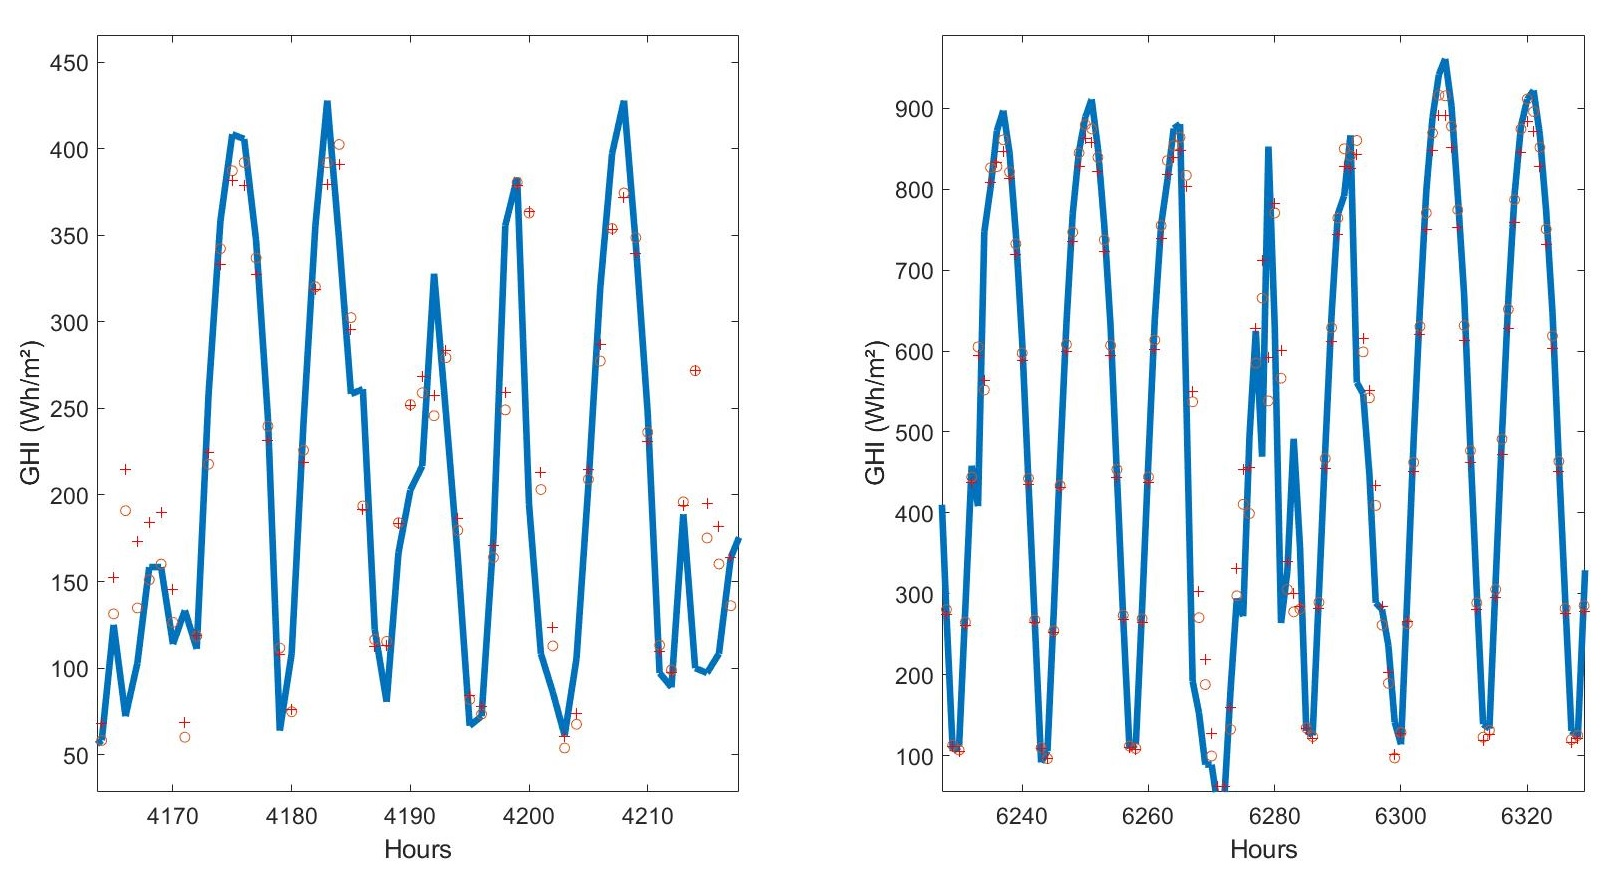
\includegraphics[scale=0.45]{fig3.jpg}% 
\caption{Prediction (1 hour horizon) for Ajaccio in winter (left) and summer (right). The blue lines correspond to the measurements (irradiation), the yellow circles to COMB, and red crosses to ARTU with $R=0.05$} 
\label{fig:fig3}
\end{figure}

\subsection{Multi-Site Study}
\label{sec:multi}
The results of the different forecasting methods are shown for four sites, one of which is relatively close to the previous one at about 105 km (Bastia). The other sites have entirely different climatological characteristics (Melbourne, Le Raizet and Nancy). The characteristics of these sites are shown in Table \ref{tab:tab2}.

\begin{table}[tb]
\centering
\begin{tabular}{@{}llrccc@{}} \toprule
	Name & Localisation & Coordinates & Alt (m) & $KG$ & $F$(\%) \\ \midrule
	\textbf{Ajaccio}    & France (Corsica)        & \begin{tabular}{@{}r@{}}41° 55' 36" N \\ 08° 44' 13" E  \end{tabular}  & 30                    & Csa         & 68            \\
	\textbf{Bastia}     & France (Corsica)        & \begin{tabular}{@{}r@{}}42° 39' 14" N \\ 09° 39' 59" E  \end{tabular}  & 30                    & Csa         & 62.1          \\ 
	\textbf{Nancy}      & France (Metropolitan)   & \begin{tabular}{@{}r@{}}48° 41' 31" N \\ 06° 11' 03" E  \end{tabular}  & 271                   & Cfb         & 50.2          \\ 
	\textbf{Le Raizet}  & France (Guadeloupe)     & \begin{tabular}{@{}r@{}}16° 16' 15" N \\ 61° 30' 16" W  \end{tabular}  & 11                    & Af          & 58.2          \\ 
    \textbf{Tilos}      & Greece                  & \begin{tabular}{@{}r@{}}36° 26' 00" N \\ 27° 22' 00" E  \end{tabular}  & 100                   & Csa         & 82.5          \\	
	\textbf{Melbourne}  & Australia               & \begin{tabular}{@{}r@{}}37° 48' 50" S \\ 144° 57' 47" E	\end{tabular}  & 31                    & Cfb         &  63.2         \\ \bottomrule
\end{tabular} 
\caption{Characteristics of the studied sites. Climate classification $KG$ according to \citet{ASCENCIOVASQUEZ2019672} and Forecastability $F$ according to \citet{doi:10.1063/5.0042710}}
\label{tab:tab2}
\end{table}

As can be seen from Table \ref{tab:tab3}, the conclusions stated in the previous Section remain valid. The climatology-persistence systematically improves the persistence and is itself systematically improved by the ARTU method. The combination of these methods (COMB) remains the best alternative according the results.

\begin{table}[tb]
\centering
\begin{tabular}{@{}llccccc@{}}
	\toprule
	          &       & \multirow{2}{*}{PER} & \multirow{2}{*}{CLIPER} & \multirow{2}{*}{ES} &           ARTU & \multirow{2}{*}{COMB} \\
	          &       &                       &                           &                     &     $R=0.05$ &                       \\ \midrule
	Ajaccio   &   &                 52.10 &                     44.45 &               46.40 &          44.27 &        \textbf{43.64} \\ \addlinespace
	Bastia    &   &                 67.28 &                     52.95 &               54.66 &          52.72 &        \textbf{52.36} \\ \addlinespace
	Nancy     &   &                 59.85 &                     59.25 &      \textbf{54.06} &          58.49 &                 54.23 \\ \addlinespace
	La Raizet &   &                 70.60 &                     51.76 &               55.03 & \textbf{51.52} &                 52.77 \\ \addlinespace
	Melbourne &   &                 66.12 &                     56.70 &               57.20 &          56.37 &        \textbf{54.52} \\ \bottomrule
\end{tabular}
\caption{Comparison of the 4 sites and results (MASE) for Ajaccio (see Section \ref{sec:ajaccio}). Error computed for all horizons comprise between 1 hour and 10 hours}
\label{tab:tab3}
\end{table}

If we focus on the site with the lowest forecastability (Nancy), Fig. \ref{fig:fig4} shows the evolution of the nRMSE and nMAE as  function of the forecast horizon and confirms that in this particular case the ES model is the most suitable. This surprising result is probably related to the fact that for this site the clear sky model is less efficient than for the others. Concerning the site with the lowest forecast errors (Melbourne), we see in Fig. \ref{fig:fig4} that COMB has good performance compared with the other models mainly over shorter horizons.

\begin{figure}[tb]
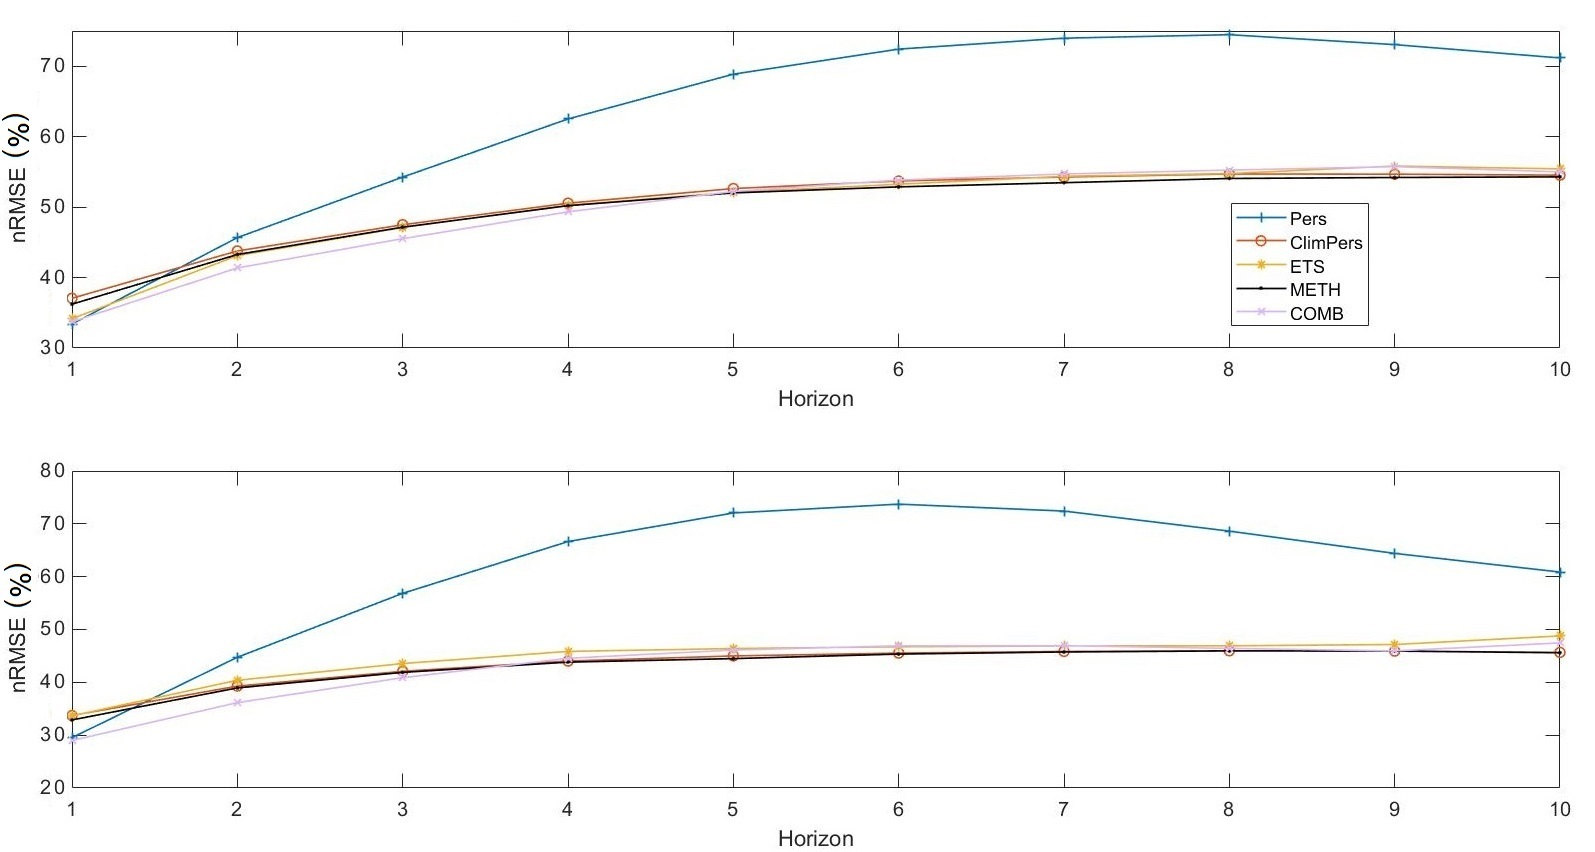
\includegraphics[scale=0.5]{fig4.jpg}% 
\caption{nRMSE evolution as function of the forecast horizon for Nancy (top) and Melbourne (bottom)} 
\label{fig:fig4}
\end{figure}

\subsection{Sensitivity to Change in Data Type}

In this Section, we study the sampling frequency of solar irradiance measurements. Moreover, here, we focus on inclined (or tilted) radiation (TGI of 30°) \citep{david_evaluating_2013}, which is generally more difficult to predict because the anistropy of the sky diffusion plays important role and is difficult to quantify. No hypothesis for the nature of radiation has been formulated in Section \ref{sec:2}; it is therefore a question of checking if the preceding conclusions are valid in this particular case. The data used were measured on the Tilos site, a small Greek island with a Mediterranean climate (36°26'00"N, 27°22'00"E, alt. 100 m). This site has a forecastability $ F =  82.5$; the data were acquired every 15 minutes and the climate of the site has a $KG$ of Csa type. For the MASE calculation, $m$ (the period in Eq.(\ref{eq:26})) was modified and taken equal to 52 ($= 13$x$4$) because there are 4 measurements per hour. The results are available in Table \ref{tab:4}.

\begin{table}[tb]
	\centering
	\begin{tabular}{@{}llccccc@{}}
		\toprule
		\multirow{2}{*}{Horizon} & \multirow{2}{*}{Metrics} & \multirow{2}{*}{PER} & \multirow{2}{*}{CLIPER} & \multirow{2}{*}{ES} &      ARTU      & \multirow{2}{*}{COMB} \\
		                         &                          &                       &                           &                     &   $R=0.05$   &                       \\ \midrule
		15 min                   & nRMSE                    &    \textbf{13.52}     &           19.27           &        24.86        &     18.71      &         14.00         \\
		                         & nMAE                     &     \textbf{6.13}     &           12.16           &        13.97        &     11.75      &         8.26          \\ \addlinespace
		75 min                   & nRMSE                    &         58.87         &           24.99           &        38.36        & \textbf{24.89} &         26.98         \\
		                         & nMAE                     &         20.91         &           15.83           &        23.15        &     15.73      &    \textbf{15.34}     \\ \addlinespace
		150 min                  & nRMSE                    &         116.9         &           25.98           &        37.55        & \textbf{25.95} &         40.17         \\
		                         & nMAE                     &         36.00         &           16.39           &        23.71        & \textbf{16.38} &         19.91         \\ \addlinespace
		                         & MASE                     &         48.49         &           33.04           &        47.52        & \textbf{32.61} &         33.04         \\ \bottomrule
	\end{tabular}
    \caption{Error metrics from the Tilos evaluation. Global tilted irradiance measured every 15 minutes.}
    \label{tab:4}
\end{table}

In this specific case, the fact that the measurements are so close together dramatically changes the results. Persistence is by far the best model for the 1-h horizon but it becomes the worst as the horizon increases. The best compromise seems to be COMB, although relatively bad at 150 min. In operations, it is not uncommon to study time steps of 15 minutes, particularly for piloting solar energy station (power or energy management system) but not up to a horizon of 150 min. In this case it will be necessary to use hourly data. Based on this observation, the COMB model is the one that provides more reliability.

\subsection{Concerning Other Meteorological Data}
\label{sec:other}
This section is dedicated to the study of meteorological time series other than solar. These are hourly series of ambient temperature \citep{CORCHADO1999351} and 10-meter wind speeds \citep{Giebel_2016}. Temperature is largely periodic and similar what we observed with solar radiation, though wind speed is entirely different and exhibits little difference between day and night. The chosen site is Nancy, already studied in Section \ref{sec:multi}. The MASE evaluation is calculated in this case with its non-periodic version. Here we quantify the importance of the stationarity of the data. Table \ref{tab:5} presents the temperature results related to the different models assuming $I_{CS}=1$ ($\forall t$). This corresponds to the non-stationary case in which $x_t$ and $\kappa_t$ are considered equal. We can expect that all models are penalized from the absence of deseasonalization of the time series, which particularly impacts ARTU.

\begin{table}[tb]
    \centering
    \begin{tabular}{@{}llccccc@{}}
        \toprule
        \multirow{2}{*}{Horizon} & \multirow{2}{*}{Metrics} & \multirow{2}{*}{PER} & \multirow{2}{*}{CLIPER} & \multirow{2}{*}{ES} &      ARTU      & \multirow{2}{*}{COMB} \\
                                 &                          &                       &                           &                     &   $R=0.05$   &                       \\ \midrule
        15 min                   & nRMSE                    &         8.90          &           8.85            &        9.03         &     17.16      &     \textbf{8.79}     \\ 
                                 & nMAE                     &         6.32          &       \textbf{6.26}       &        6.45         &     13.59      &         6.35          \\ \addlinespace
        75 min                   & nRMSE                    &         27.91         &           26.21           &        27.16        &     26.25      &    \textbf{26.13}     \\ 
                                 & nMAE                     &         21.90         &           20.36           &        21.60        & \textbf{20.07} &         20.30         \\ \addlinespace
        150 min                  & nRMSE                    &         39.28         &           34.36           &   \textbf{29.36}    &     30.67      &         31.45         \\ 
                                 & nMAE                     &         33.62         &           28.17           &        25.09        & \textbf{24.80} &         26.39         \\ \addlinespace
                                 & MASE                     &         352.4         &           310.9           &        312.5        & \textbf{290.9} &         307.2         \\ \bottomrule
    \end{tabular}
    \caption{Error metrics from the temperature evaluation without seasonal adjustments.}
    \label{tab:5}
\end{table}



 The results do not correspond to what we have observed so far. The dynamic range of the signal tested is very low and the regularity of the successive measurements make it a good candidate for the use of persistence. Although the results are not good for the very short-term horizons; ARTU remains the method which is the most efficient on average. However, given its simplicity and the very good results observed in the first horizons, ES is undoubtedly the reference method that should be used to properly characterize temperature forecasts. This suggests that as soon as the signal is regular with low variability, the forecast reference must imperatively be made with exponential smoothing. If we now focus on the estimation of wind speeds (Table \ref{tab:6} still considering $I_{CS}=1$), the conclusions are different yet not inconsistent given the large difference in variability between these two meteorological quantities. 

\begin{table}[tb]
\centering
    \begin{tabular}{@{}llccccc@{}}
        \toprule
        \multirow{2}{*}{Horizon} & \multirow{2}{*}{Metrics} & \multirow{2}{*}{PER} & \multirow{2}{*}{CLIPER} & \multirow{2}{*}{ES} &      ARTU      & \multirow{2}{*}{COMB} \\
                                 &                          &                       &                           &                     &   $R=0.05$   &                       \\ \midrule
        15 min                   & nRMSE                    &         46.47         &      \textbf{41.78}       &        44.28        &     47.00      &         42.33         \\ 
                                 & nMAE                     &         31.98         &      \textbf{30.18}       &        32.19        &     34.62      &         30.47         \\ \addlinespace
        75 min                   & nRMSE                    &         70.23         &           52.67           &        53.59        & \textbf{52.65} &         54.22         \\ 
                                 & nMAE                     &         53.22         &           39.42           &        40.12        & \textbf{39.39} &         40.85         \\ \addlinespace
        150 min                  & nRMSE                    &         73.73         &      \textbf{53.04}       &        53.96        &     53.16      &         55.10         \\ 
                                 & nMAE                     &         56.31         &      \textbf{39.53}       &        40.49        &     39.58      &         41.50         \\ \addlinespace
                                 & MASE                     &         159.6         &           120.2           &        122.9        & \textbf{120.2} &         124.5         \\ \bottomrule
    \end{tabular}
\caption{Error metrics concerning the wind speed evaluation without seasonal adjustments.}
\label{tab:6}
\end{table}

We observed that the climatology-persistence performed well in the case of solar radiation and its prediction. We see here that this is the best of the tested models and undoubtedly the easiest to set up. The ARTU model gives fairly comparable results. If, in the case of temperature, the ACF values were close from one lag to another, here it is the reverse; the correlations become insignificantly different from 0 very quickly. We observe an exponential decay (see Section \ref{sec:method}), which suggests that the best model is indeed an AR(1) and therefore it is not surprising that CLIPER performs best and that ARTU does not bring a real added value to this case.  

Using $I_{CS}$ as defined in Section \ref{sec:season} with the time decomposition, we are able to see the impact of seasonal adjustment on the results. Tables \ref{tab:7} and \ref{tab:8} show the results according the temperature and the wind speed, respectively.

\begin{table}[tb]
\centering
    \begin{tabular}{@{}llccccc@{}}
    	\toprule
    	\multirow{2}{*}{Horizon} & \multirow{2}{*}{Metrics} & \multirow{2}{*}{PER} & \multirow{2}{*}{CLIPER} & \multirow{2}{*}{ES} &      ARTU      & \multirow{2}{*}{COMB} \\
    	                         &                          &                       &                           &                     &   $R=0.05$   &                       \\ \midrule	
    	15 min                   & nRMSE                    &         6.08          &       \textbf{5.91}       &        6.19         &      6.85      &         6.02          \\ 
    	                         & nMAE                     &     \textbf{4.01}     &           4.03            &        4.17         &      5.02      &         4.06          \\ \addlinespace
    	75 min                   & nRMSE                    &         14.66         &           12.19           &        13.86        & \textbf{12.17} &         12.82         \\ 
    	                         & nMAE                     &         10.25         &           9.06            &        9.82         & \textbf{9.06}  &         9.23          \\ \addlinespace
    	150 min                  & nRMSE                    &         19.62         &           14.07           &        14.66        & \textbf{13.12} &         14.44         \\ 
    	                         & nMAE                     &         14.01         &           10.74           &        11.01        & \textbf{9.96}  &         10.87         \\ \addlinespace
    	                         & MASE                     &         149.5         &           131.8           &        134.5        & \textbf{129.3} &         130.8         \\ \bottomrule
    \end{tabular}
\caption{Error metrics concerning the temperature evaluation with seasonal adjustments.}
\label{tab:7}
\end{table}

Even though this result has been understood for some time, we measure the importance of the ratio to trend and of the seasonal adjustment with these 2 Tables. The temperature results are very good for all methods and particularly for ARTU (nMAE$=9.96$ for a 10-h horizon). It is likely that few machine-learning methods can significantly improve this result. For wind speeds, CLIPER remains the best way to make simple forecasts, even if ARTU and COMB can be very interesting alternatives, but also more complicated to set up.

\begin{table} [!htb]
\centering
    \begin{tabular}{@{}llccccc@{}}
    	\toprule
    	\multirow{2}{*}{Horizon} & \multirow{2}{*}{Metrics} & \multirow{2}{*}{PER} & \multirow{2}{*}{CLIPER} & \multirow{2}{*}{ES} &      ARTU      & \multirow{2}{*}{COMB} \\
    	                         &                          &                       &                           &                     &   $R=0.05$   &                       \\ \midrule	
    	15 min                   & nRMSE                    &         39.87         &           35.11           &        36.30        &     34.95      &    \textbf{34.90}     \\ 
    	                         & nMAE                     &         28.64         &           25.41           &        26.14        &     25.30      &    \textbf{25.18}     \\ \addlinespace
    	75 min                   & nRMSE                    &         55.21         &      \textbf{41.32}       &        42.24        &     41.33      &         42.10         \\ 
    	                         & nMAE                     &         39.91         &           29.70           &        30.59        & \textbf{29.69} &         30.51         \\ \addlinespace
    	150 min                  & nRMSE                    &         58.53         &      \textbf{42.07}       &        42.85        &     42.26      &         43.31         \\ 
    	                         & nMAE                     &         42.79         &      \textbf{30.09}       &        30.84        &     30.21      &         31.30         \\ \addlinespace
    	                         & MASE                     &         118.8         &           90.0            &        91.4         & \textbf{89.7}  &         91.7          \\ \bottomrule
    \end{tabular}
\caption{Error metrics concerning the wind speed evaluation with seasonal adjustments.}
\label{tab:8}
\end{table}

The field of wind forecasting is a very particular and complicated discipline. The choice to use the mean to try to make the series stationary is simple to establish though is perhaps not the best approach should we seek better results. Though not mentioned here, single, double or seasonal differencing would all have the effect of improving stationarity.
